\subsection*{Memory}
\underline{RAM/ROM:}\\
\begin{minipage}{.49\columnwidth}
    \centering
    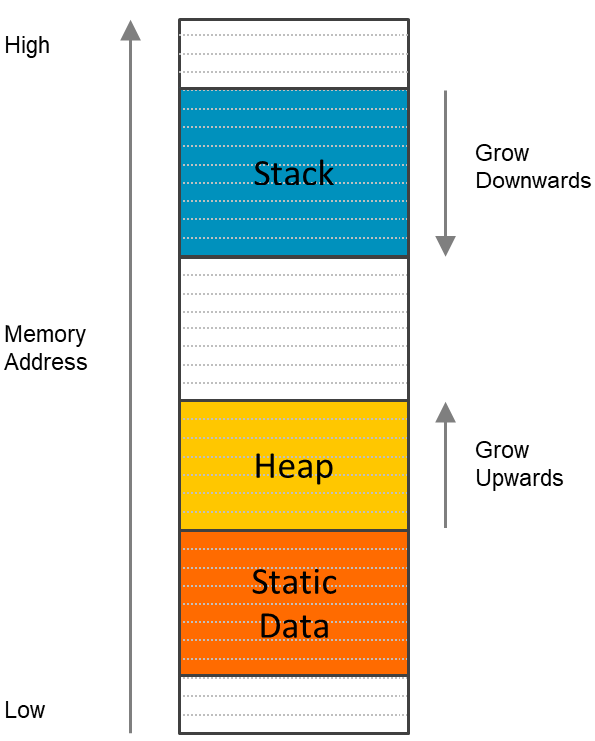
\includegraphics[width=\linewidth]{images/ram1.png}
\end{minipage}
\begin{minipage}{.49\columnwidth}
    \centering
    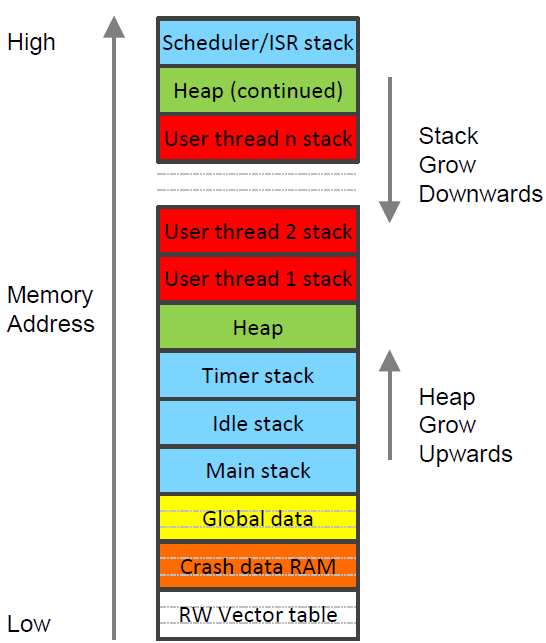
\includegraphics[width=\linewidth,height=\linewidth,keepaspectratio=false]{images/ram2.png} % set height to \linewidth
\end{minipage}\\
Typically, the data can be divided into three
sections: static data, stack, and heap:
\begin{itemize}
    \item Static data: contains global variables and static variables
    \item Stack: contains the temporary data for local variables, parameter passing in function calls, registers saving during exceptions, etc.
    \item Heap: contains the pieces of memory spaces that are dynamically reserved by calloc() malloc() or new calls.
\end{itemize}
\includegraphics*[width=\columnwidth]{images/datastorage_example.png}
Can the information change?
\begin{itemize}
    \item No: put it in read-only, nonvolatile memory for saving RAM
    \item Yes: put it in read/write memory
\end{itemize}
How long does the data need to exist?
\begin{itemize}
    \item Program scope: statically allocated
    \item Function/method scope: automatically allocated on the stack
    \item From explicit allocation to explicit deallocation: on the heap
    \item Always define the most restrictive scope
    \item Use dynamic allocation on the heap with care
\end{itemize}
\underline{Class qualifiers and data type:}\\
\includegraphics*[width=\columnwidth]{images/data_types.png}
\begin{itemize}
    \item \texttt{const}: the value of the variable cannot be changed after initialization.
          Never written by program, can be put in ROM to save RAM.
    \item \texttt{volatile}: the value of the variable can be changed by external events.
          Can be changed outside of normal program flow: ISR, hardware register
          Compiler must be careful with optimizations.
    \item \texttt{static}: the variable is shared between all instances of the class.
          Declared within function or method, retains value between function/method invocations
          Declared within classes: the field is instantiated once for all class instances and the value
          is retained for the program lifetime.
\end{itemize}
\underline{Memory hierarchy:}\\
\includegraphics*[width=\columnwidth]{images/memory_hierarchy.png}
\begin{itemize}[itemsep=0pt, topsep=0pt, partopsep=0pt]
    \item Register: usually one CPU cycle to access
    \item Cache: Static RAM
    \item Main Memory: Dynamic RAM, Volatile data
    \item Secondary Memory: Flash/Hard disk
    \item Tertiary Memory: Tape libraries
\end{itemize}